\section{Durchführung}
\label{sec:Durchführung}
Der generelle Plan zur Bestimmung der Suszeptibilität, ist nun ein Wechselstromsignal an eine
Brückenschaltung aus Induktivitäten anzulegen. Die Brückenschaltung soll dann abgeglichen werden, woraufhin eine Probe eines
Materials in eine Spule geschoben wird und ihre Induktivität vergrößert. Gemessen werden soll dann die resultierende Brückenspannung
und das neue Abgleichverhältnis der Widerstände. Das generelle Problem dabei besteht darin, dass die Spannungssignale, die durch einführen der Suszeptibilität entstehen,
so klein sind, dass sie sich nicht klar vom generellen Rauschen abheben. Deswegen wird wie in Abbildung \ref{fig:Messung}
ein Selektivverstärker vor das Millivoltmeter geschaltet, der nur bestimmte Frequenzen durchlässt, wodurch nur die Signalfrequenz ohne das Rauschen verstärkt wird und so gemessen werden kann. Nun soll als erstes die
Durchlasskurve dieses Geräts bestimmt werden. Also es soll bestimmt werden welcher Anteil der Eingangsspannung am Ausgang ankommt.
Dafür wird ein Signalgenerator an den Selektivverstärker angeschlossen der Sinussignale zwischen 20-40 kHz ausgeben soll.
Der Ausgang des Verstärkers wird auf ein Oszilloskop gegeben, sodass die Amplitudenspannung gut ablesbar ist. Nun werden 30 Messpunkte im Intervall
genommen, wobei im Bereich der maximalen Spannung die meisten Messwerte genommen werden.\\

\noindent Nun kann der Signalgenerator auf die Frequenz mit optimalen Durchlass eingestellt werden.
Das Signal wird nun erst als Speisespannung auf die Brückenschaltung gegeben. Die Brückenspannung wird abgegriffen auf den Selektivverstärker gegeben.
Das selektierte und verstärkte Signal wird an einem Millivoltmeter gemessen. Nun wird zuerst das Widerstandsverhältnis so eingestellt, dass die Brücke abgeglichen ist, sodass
die Brückenspannung verschwindet. Nun wird die Probe eines Materials in eine Spule geschoben. Nun unterscheidet sich die Brückenspannung wieder
von 0 und kann gemessen werden. Zusätzlich wird nun die Brücke inklusive Probe abgeglichen und das neue
Widerstandsverhältnis notiert. Nun wird die Probe wieder entfernt und die Brücke wird erneut im Grundzustand abgeglichen und das Widerstandsverhältnis wird auch dort notiert.
Der Vorgang wird dreimal für jede Probe wiederholt. Es werden die Proben \ce{Nd2O3},\ce{Gd2O3} und \ce{Dy2O3} untersucht.
Als letztes müssen noch einige geometrische Größen wie die Länge der Probe genommen werden.
\begin{figure}[H]
    \centering
    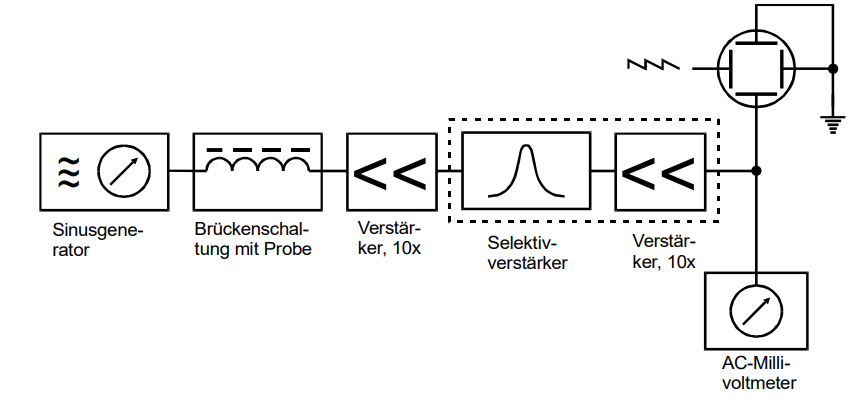
\includegraphics[scale=0.7]{content/Messschaltung.png}
    \caption{Selektivverstärkung des Signals.}
    \label{fig:Messung}
\end{figure}
